%%%%%%%%%%%%%%%%%%%%%%%%%%%%%%%%%%%%%%%%%%%%%%%%%%%%%%%%%%%%%%%%%%%%%%%%%%
%%%%%                        Intro Générale                         %%%%%%
%%%%%%%%%%%%%%%%%%%%%%%%%%%%%%%%%%%%%%%%%%%%%%%%%%%%%%%%%%%%%%%%%%%%%%%%%%
\phantomsection
\addcontentsline{toc}{chapter}{Introduction générale}
\addtocontents{toc}{\protect\addvspace{10pt}}

\lhead[\fancyplain{}{Introduction générale}]
      {\fancyplain{}{}}
\chead[\fancyplain{}{}]
      {\fancyplain{}{}}
\rhead[\fancyplain{}{}]
      {\fancyplain{}{Introduction générale}}
\lfoot[\fancyplain{}{}]%
      {\fancyplain{}{}}
\cfoot[\fancyplain{}{\thepage}]
      {\fancyplain{}{\thepage}}
\rfoot[\fancyplain{}{}]%
     {\fancyplain{}{\scriptsize}}
     
\thispagestyle{plain}

%%%%%%%%%%%%%%%%%%%%%%%%%%%%%%%%%%%%%%%%%%%%%%%%%%%%%%%%%%%%%%%%%%%%%%%%%%
%%%%%                      Start part here                          %%%%%%
%%%%%%%%%%%%%%%%%%%%%%%%%%%%%%%%%%%%%%%%%%%%%%%%%%%%%%%%%%%%%%%%%%%%%%%%%%

\chapter*{\lettrine[lines=1]{I}{ntroduction générale}}
\label{ch/introduction}

\vspace{1.5cm}

La turbulence est un état particulier d'un écoulement qui se caractérise par la formation, la régénération et la coexistence de structures tourbillonnaires dont la taille varie de l'échelle de Kolmogorov aux grandes structures énergétiques. Les écoulements turbulents s'observent partout, que ce soit lors de la cuisson des pâtes, en course automobile ou avec les courants atmosphériques. Ils ont un impact non négligeable d'un point de vue industriel. Par exemple, la puissance motrice vient combattre la force de traînée induite par les différentes échelles de la turbulence dans le secteur de l'aéronautique. Néanmoins, il existe des exemples dans lesquels la turbulence est bénéfique, car elle augmente significativement le mélange (\cite{Dimotakis2005}) et le transfert thermique pariétal. Elle permet également de transporter rapidement de l’énergie et de la chaleur d’un endroit à un autre. Le micromélange turbulent d'un scalaire passif couvre toutes les échelles spatiotemporelles d’un écoulement turbulent (\cite{Eckart1948, Yakhot2008}). C’est le cas notamment pour la dispersion et le mélange de traceurs (polluant, fumée, nuage de petites particules, encre ou colorant alimentaires). Le mélange est actif et couplé à la dynamique dans les cas les plus complexes, comme pour le mélange de fluide de densités différentes dans les courants atmosphériques, le mélange de température (ou de salinité) dans les courants océaniques, ou le transport sédimentaire. Enfin, le mélange induit un changement des propriétés du fluide (densité, pression, enthalpie, etc.) dans les cas les plus extrêmes comme dans la combustion.\\

Le contrôle des écoulements relève d'un fort intérêt économique et de performance des systèmes et des procédés concernés. L'optimisation des processus reposant sur des principes de mélange ou de transferts thermiques permet, par exemple, d'améliorer la performance des échangeurs. L'amélioration des transferts thermiques revient alors à réduire la résistance thermique, soit en augmentant la surface effective du transfert, soit en manipulant intrinsèquement l'écoulement. Les échangeurs thermiques sont présents dans beaucoup de secteurs de l'industrie : microélectronique, nucléaire, médical, bâtiment, automobile, et bien d'autres (\cite{Mousa2021}). Les méthodes pour améliorer les échanges thermiques se distinguent en deux groupes : les méthodes actives et passives. Les méthodes actives requièrent de l'énergie pour contrôler, en temps réel, la turbulence et les transferts thermiques qui en découlent. C'est le cas, entre autres, des contrôles par électrohydrodynamique (EHD) ou magnétohydrodynamique (MHD). Les méthodes passives ne requièrent pas d'énergie et consistent, par exemple, en une modification de la paroi ou l'ajout de dispositifs statiques dans l'écoulement. C'est le cas notamment des géométries torsadées ou hélicoïdales, des déflecteurs ou générateurs de tourbillons et des parois rugueuses. Le lecteur intéressé pourra se référer aux études bibliographiques de \cite{Sheikholeslami2015} et de \cite{Maradiya2018}. L'optimisation des échangeurs thermiques peut mener à une réduction de l'utilisation des matériaux qui les composent ou des déchets qu'ils engendrent suite à une défaillance, voire à une réduction de l'énergie qu'ils consomment. Cela pourrait aussi les rendre plus compacts et donc augmenter leurs rendements surfaciques. En mettant de côté les transferts thermiques, l'augmentation du mélange d'un scalaire passif peut aussi trouver un intérêt dans le domaine médical comme le séquençage de l'ADN ou l'administration de médicaments dans le sang, ainsi que dans le domaine de la papeterie avec l'impression à jet d'encre. Enfin, avec les avancées constantes en microtechnologie, de plus en plus de systèmes biomédicaux, chimiques et électroniques sont miniaturisés. Les problématiques liées à la surchauffe des éléments, du matériel informatique (CPUs, GPUs, datacenters, puces électroniques) ou de systèmes micro-électromécaniques (MEMS) vont donc être de plus en plus primordiales. La génération de chaleur et la surchauffe des composants impactent de manière non négligeable leur durée de vie et les conséquences vont d’une baisse de performance à une défaillance totale.\\

La turbulence est un excellent mélangeur. Le mélange d'un scalaire passif dans un écoulement en présence de parois est meilleur dans le régime turbulent, comparé aux régimes laminaires et chaotiques (\cite{Kadoch2020}). Le processus de transfert de chaleur à la paroi est de même plus performant en écoulements turbulents qu'en écoulements chaotiques. Ce gain en performance est, en revanche, contrecarrée par l'augmentation des pertes de charges. Il existe cependant des applications pour lesquelles le dernier point est moins important, et le mélange et le transfert thermique pariétal sont primordiaux. L'ingénieur a donc tout intérêt à travailler avec un écoulement turbulent lorsque ceci s'avère possible, voire à imiter la turbulence pariétale par un contrôle actif. Il existe en effet certains procédés dans lesquels les structures tourbillonnaires similaires à celles d'un écoulement turbulent développé sont provoquées en imposant un forçage spécifique et qui localement améliorent le mélange à des nombres de Reynolds particulièrement faible (\cite{Tardu2012}).\\

Cette thèse a été, à l'origine, motivée par la problématique de refroidissement des lasers à ultra-haute intensité. En effet, cette technologie connaît un fort essor grâce à la maîtrise de la technique d'amplification d'impulsions à dérive de fréquence (CPA) mise au point par Gérard Mourou (\citet{Strickland1985}). Des lasers multi-pétawatts peuvent être utilisés à haute fréquence à condition de maîtriser le refroidissement des amplificateurs, car la répétition du laser en provoque leur surchauffe. Il est donc nécessaire d’évacuer l'accumulation de chaleur, par convection forcée. Le refroidissement s’opère donc avec un fluide passant entre deux amplificateurs, ce qui s’apparente à un écoulement en canal. Un point important à préciser et qu’un écoulement turbulent altère la qualité du faisceau du laser en brouillant sa phase (\cite{Bellec2019}). C'est pourquoi, le refroidissement par convection forcée se fait, à présent, avec un écoulement laminaire, ce qui est nettement moins efficace au niveau échange thermique comparé à la convection forcée turbulente. Il faut envisager un dispositif (si possible) passif de contrôle afin d'améliorer le processus de transfert thermique et de piloter les caractéristiques du mélange. M. Alain Girard, du département des systèmes à basse température du CEA-Grenoble et co-encadrant de cette thèse, a organisé plusieurs réunions il y a maintenant quelques années sur la thématique du refroidissement des lasers à ultra-haute intensité. Lors d'une de ces réunions, le LEGI a proposé de répartir des rugosités avec une distribution spécifique et particulière dans la zone de développement hydraulique d'un écoulement en canal initialement laminaire (\cref{fig/fig_intro}). L'objectif serait alors de déclencher une transition de type bypass, rapide et efficace dans la zone d'entrée hydraulique pour améliorer le processus de transfert dans l'écoulement développé qui suit. La zone non manipulée de la \cref{fig/fig_intro} représente l'amplificateur laser dans lequel aucune intervention n'est possible. Il est donc impératif d'agir en amont. Une autre particularité de la proposition fut que le nombre de Reynolds soit aux alentours du nombre de Reynolds critique $Re_{cr}$ (nombre de Reynolds en dessous duquel la turbulence ne survit pas) et que l’écoulement initial soit laminaire. En effet, ce procédé pourrait alors trouver d'autres applications comme en microfluidique où le nombre de $Re$ est faible.\\

\vspace{3cm}
\begin{figure}[!hbtp]
    \centering
    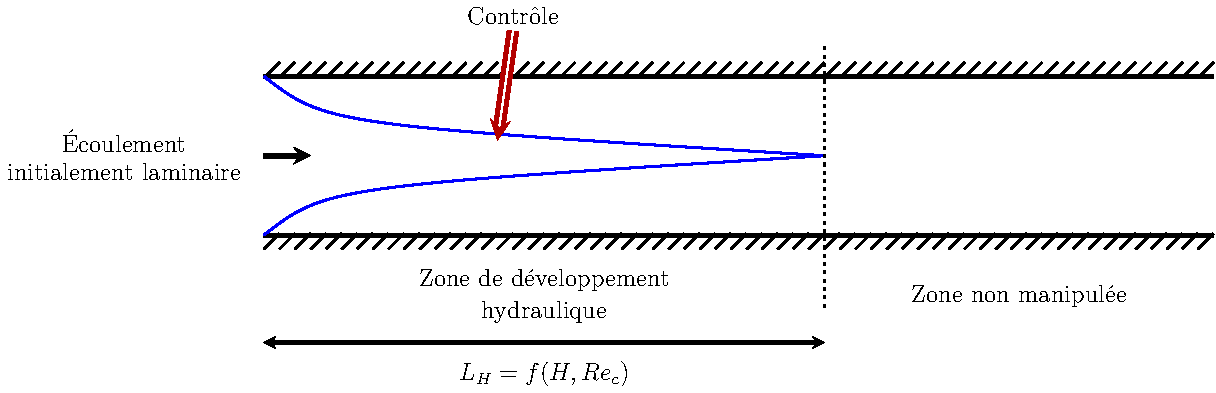
\includegraphics[width=\linewidth]{Intro/Pictures/Figure_intro.pdf}
    \caption{Contrôle passif appliqué à la zone de développement hydraulique d'un écoulement en canal initialement laminaire.}
    \label{fig/fig_intro}
\end{figure}

\clearpage
La zone de développement hydraulique n’a pas reçu suffisamment d’attention dans la littérature. Mis à part l'étude de \cite{Buffat2014}, il n'y a pas d'investigation sur la transition bypass dans cette région, et moins encore sur le transport d'un scalaire passif. La littérature sur la structure dynamique d'un spot transitionnel dans un écoulement de Poiseuille est très riche. Il y a cependant une carence en ce qui concerne le transport d'un scalaire passif au sein d'un spot dans la littérature. Une partie de cette recherche est donc dédiée à combler cette carence, ne serait-ce que partiellement. Ce thème paraît au premier abord découplé du reste du manuscrit qui se compose donc en deux parties plus ou moins indépendantes. Il faut souligner cependant que certaines étapes de la transition bypass déclenchée par des rugosités en quinconce contiennent des spots locaux similaires à ce qui est observé dans un écoulement de Poiseuille (\cite{Anika2020}). Le \cref{ch/biblio} de cette thèse vise à poser le cadre du travail ci-présent à travers un exposé sur l'état de l'art sur la transition bypass et les écoulements rugueux. Le \cref{ch/DNS} présente le code de simulations numériques directes (SND). Un temps non négligeable a été consacré à l'implémentation des méthodes comme celle de \foreignquote{french}{Fringe} et des frontières immergées qui n'existaient pas dans le code initial. Le chapitre 3 est consacré au transport d'un scalaire passif au sein d'un spot transitionnel. L'effet des rugosités en quinconce sur la transition bypass, la dynamique et le scalaire passif est analysé dans le chapitre 4. Une étude paramétrique est menée dans ce dernier afin d'élucider l'effet de la distribution géométrique des rugosités sur l'établissement d'un régime pseudo-rugueux, dans un écoulement initialement laminaire à un nombre de $Re$ particulièrement faible. Enfin, le chapitre 5 s'intéresse à l'impact des rugosités dans la zone de développement hydraulique sur la zone développée, conformément à l'objectif principal de cette étude. Le lecteur remarquera qu'une nouvelle approche numérique de sous-domaines interconnectés a été mis en place afin d'effectuer des SND à coût raisonnable dans ce domaine particulièrement large.
